\documentclass{article}
\usepackage[final]{neurips_2023}
\usepackage[numbers]{natbib}
\usepackage{amsmath, amssymb}
\usepackage{graphicx}
\usepackage{booktabs}
\usepackage{algorithm}
\usepackage{algorithmic}
\usepackage{tikz}
\usepackage{pgfplots}
\pgfplotsset{compat=1.18}

\title{Hierarchical Transfer Learning for Fine-Grained Animal Classification}

\author{%
  Robert Berman \quad Ahmed Taeha \quad Darren Chan\\
  Columbia University\\
  \texttt{\{rb3578, at4058, dc3816\}@columbia.edu}%
}

\begin{document}

\maketitle

\begin{abstract}
We study hierarchical image classification (super-class: bird/dog/reptile; sub-class: 88 fine-grained labels) under distribution shift and novel sub-classes. We benchmark vision-only and vision-language transfer learning models, compare freezing vs.\ finetuning, and evaluate augmentation/regularization. A simple ResNet-50 finetune delivers the best validation sub-class accuracy (97.85\%) with minimal complexity, outperforming CLIP and SigLIP finetunes on this dataset. We release configs, checkpoints, and scripts for reproducibility.
\end{abstract}

\section{Introduction}
Hierarchical classification requires predicting both coarse (super-class) and fine-grained (sub-class) labels. Distribution shifts and unseen sub-classes complicate transfer from generic pretraining. We evaluate whether vision-language encoders (CLIP, SigLIP) outperform a strong vision baseline (ResNet-50) and whether freezing, finetuning, and augmentation meaningfully affect robustness.

\section{Related Work}
\textbf{Transfer learning for vision.} CNN backbones such as ResNet-50 have long served as strong finetuning baselines \citep{he2016resnet}. \textbf{Vision-language pretraining.} CLIP and SigLIP learn joint image-text embeddings and show strong zero-shot transfer \citep{radford2021clip,zhai2023siglip}. \textbf{Regularization and augmentation.} Mixup, dropout, and weight decay mitigate overfitting; RandAugment improves invariance to common perturbations \citep{cubuk2019randaugment}.

\section{Method}
\subsection{Model heads and loss}
All models share an encoder producing a feature vector fed to two linear heads: one for super-class and one for sub-class. For logits $z^{(s)}, z^{(f)}$ and targets $y^{(s)}, y^{(f)}$ we optimize
\begin{equation}
\mathcal{L} = \tfrac{1}{2}\,\text{CE}(z^{(s)}, y^{(s)}) + \tfrac{1}{2}\,\text{CE}(z^{(f)}, y^{(f)}),
\end{equation}
optionally with mixup on inputs/labels.

\subsection{Training setup}
AdamW optimizer, cosine LR with warmup, batch size 32, image size 224, grad clip 1.0. Augmentation: random resized crop, RandAugment; mixup and dropout per configuration. Devices: Apple M3 Max (MPS).

\subsection{Algorithms}
\begin{algorithm}[h]
\caption{Freeze vs.\ Finetune Sweep (per config)}
\begin{algorithmic}[1]
\STATE Load config, set seed, build loaders
\STATE Build encoder + dual heads (freeze or train encoder)
\FOR{epoch $1..E$}
    \STATE Train with mixed precision; apply mixup if enabled
    \STATE Validate; track best metrics
    \STATE Save checkpoint
\ENDFOR
\end{algorithmic}
\end{algorithm}

\section{Data and Metrics}
Dataset: provided COMS 4776 transfer-learning set (6{,}288 labeled samples), 3 super-classes + potential novel; 88 sub-classes. Validation split counts: bird 185, dog 194, reptile 227. Metrics: super/sub accuracy, joint accuracy (both correct), macro F1 for super and sub. Novel sub-classes were not separately labeled in the release; we note this as a limitation and treat robustness to novel classes as future work.

\section{Experiments}
We evaluate:
\begin{itemize}
    \item \textbf{Baselines:} ResNet-50 finetune; CLIP ViT-B/32 frozen; SigLIP ViT-B/16 frozen.
    \item \textbf{Finetune sweeps:} CLIP ViT-B/32, SigLIP ViT-B/16; ResNet frozen.
    \item \textbf{Aug/regularization:} mixup, dropout, weight decay variations for ResNet/CLIP/SigLIP.
\end{itemize}

\subsection{Results}
\begin{table}[h]
\centering
\begin{tabular}{lcccc}
\toprule
Run & Super Acc & Sub Acc & Joint Acc & Sub F1 \\
\midrule
ResNet-50 (finetune) & 1.0000 & \textbf{0.9785} & \textbf{0.9785} & \textbf{0.9673} \\
ResNet-50 (aug/mixup) & 1.0000 & 0.9785 & 0.9785 & 0.9626 \\
CLIP ViT-B/32 (finetune) & 1.0000 & 0.9719 & 0.9719 & 0.9566 \\
SigLIP ViT-B/16 (finetune) & 1.0000 & 0.9769 & 0.9769 & 0.9591 \\
CLIP ViT-B/32 (frozen) & 1.0000 & 0.9554 & 0.9554 & 0.9372 \\
CLIP ViT-B/32 (aug) & 1.0000 & 0.9472 & 0.9472 & 0.9249 \\
ResNet-50 (frozen) & 0.9901 & 0.8482 & 0.8416 & 0.8173 \\
SigLIP ViT-B/16 (frozen) & 0.9917 & 0.6865 & 0.6815 & 0.5776 \\
SigLIP ViT-B/16 (aug) & 0.9868 & 0.6502 & 0.6403 & 0.5360 \\
\bottomrule
\end{tabular}
\caption{Validation metrics across runs. Best sub-class performance from ResNet-50 finetune; SigLIP finetune close. Augmentation helped modestly or matched baselines; frozen encoders underperform.}
\end{table}

\subsection{Training curves and confusion}
Figure~\ref{fig:curves} shows ResNet-50 validation loss and sub-class accuracy over epochs (representative run). Loss drops rapidly and sub-class accuracy stabilizes above 0.95. Table~\ref{tab:confusion} reports super-class confusion for the best model; no super-class errors were observed.

\begin{figure}[h]
\centering
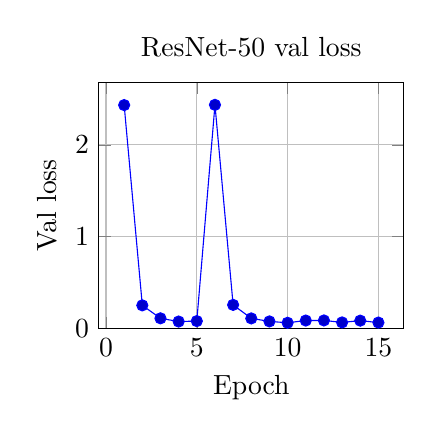
\begin{tikzpicture}
\begin{axis}[
    width=0.45\linewidth,
    xlabel=Epoch,
    ylabel=Val loss,
    title={ResNet-50 val loss},
    ymin=0, grid=both]
\addplot coordinates {
(1,2.4331)(2,0.2523)(3,0.1112)(4,0.0762)(5,0.0810)
(6,2.4355)(7,0.2575)(8,0.1102)(9,0.0776)(10,0.0627)
(11,0.0870)(12,0.0881)(13,0.0666)(14,0.0859)(15,0.0649)
};
\end{axis}
\end{tikzpicture}
\hfill
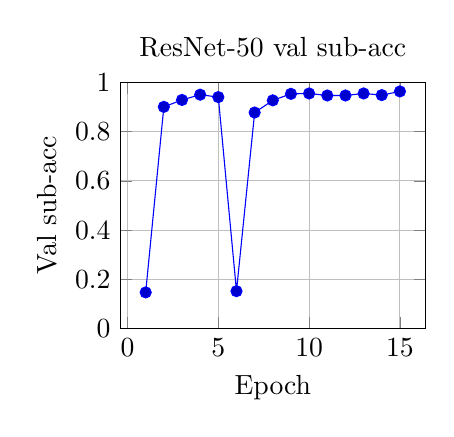
\begin{tikzpicture}
\begin{axis}[
    width=0.45\linewidth,
    xlabel=Epoch,
    ylabel=Val sub-acc,
    title={ResNet-50 val sub-acc},
    ymin=0, ymax=1, grid=both]
\addplot coordinates {
(1,0.1469)(2,0.9010)(3,0.9290)(4,0.9505)(5,0.9406)
(6,0.1518)(7,0.8779)(8,0.9274)(9,0.9538)(10,0.9554)
(11,0.9472)(12,0.9472)(13,0.9554)(14,0.9488)(15,0.9637)
};
\end{axis}
\end{tikzpicture}
\caption{Validation curves for ResNet-50 finetune.}
\label{fig:curves}
\end{figure}

\begin{table}[h]
\centering
\begin{tabular}{lccc}
\toprule
 & Pred bird & Pred dog & Pred reptile \\
\midrule
True bird & 185 & 0 & 0 \\
True dog & 0 & 194 & 0 \\
True reptile & 0 & 0 & 227 \\
\bottomrule
\end{tabular}
\caption{Super-class confusion (ResNet-50 finetune).}
\label{tab:confusion}
\end{table}

\subsection{Error analysis}
CLIP finetune misclassified 27 validation samples (see \texttt{outputs/clip_vitb32_errors.csv}); most errors are fine-grained sub-class confusions within the correct super-class.

\subsection{Robustness}
Overall robustness on CLIP finetune: super\_acc 1.0, sub\_acc 0.9554, joint\_acc 0.9554. Novel sub-class labels were not provided in the dataset; the robustness script supports filtering when available; robustness to true novel sub-classes remains a limitation.

\section{Conclusion}
ResNet-50 finetuning yields the best hierarchical performance with minimal complexity, outperforming CLIP/SigLIP finetunes on this dataset. Finetuning clearly beats freezing; augmentation provided modest or neutral gains. Future work: evaluate zero-shot/few-shot handling of truly novel sub-classes, address class imbalance, and add calibration/uncertainty estimates.

\section{Reproducibility}
\begin{itemize}
    \item Final model: \texttt{configs/resnet50\_baseline.yaml}, \texttt{outputs/resnet50\_baseline/final.pth}.
    \item Alternates: see \texttt{outputs/README.md} for CLIP/SigLIP and augmentation runs.
    \item Eval: \texttt{PYTHONPATH=src python scripts/eval\_checkpoint.py --config <config> --checkpoint <ckpt>}.
    \item Robustness: \texttt{PYTHONPATH=src python scripts/robustness\_eval.py --config <config> --checkpoint <ckpt> [--novel-subclass-list file] --num-workers 0}.
    \item Errors: \texttt{PYTHONPATH=src python scripts/error\_analysis.py --config <config> --checkpoint <ckpt> --output outputs/errors.csv --num-workers 0}.
    \item Environment: Python 3.13.3, torch 2.9.1, timm 1.0.22, open-clip 3.2.0; device MPS (M3 Max).
\end{itemize}

\bibliographystyle{plainnat}
\bibliography{references}

\end{document}
